\subsection{Desarrollo del proyecto}
El desarrollo de la aplicación web SHIFTLY se realizó mediante un proceso
de trabajo colaborativo. Cada integrante del equipo recibió diferentes
interfaces y funcionalidades para desarrollar de acuerdo con la
distribución establecida mediante las actividades del proyecto.
\subsection{Desarrollo de interfaces}
A continuación se documentan las principales interfaces desarrolladas por
cada integrante del equipo, indicando la función de cada una y su
participación dentro del proyecto
\subsubsection{Registro de usuario}
\textbf{Descripción}
La interfaz de registro de usuario permite crear una cuenta en SHIFTLY
para acceder a la plataforma de aprendizaje de inglés. La pantalla
presenta un formulario de registro organizado en una tarjeta central, con
los elementos necesarios para introducir la información del usuario.
\textbf{Barra de navegación}
La parte superior de la interfaz contiene la identidad visual de SHIFTLY,
representada mediante el logotipo y el nombre de la aplicación. En la
parte derecha se encuentra la opción ``Iniciar Sesión'', destinada a los
usuarios que ya cuentan con una cuenta.
\textbf{Encabezado del formulario}
El formulario presenta el texto ``EMPIEZA HOY'' como encabezado y el título
``Crear Cuenta''. También incluye un mensaje introductorio que invita al
usuario a registrarse en SHIFTLY para comenzar su aprendizaje.
\textbf{Campos de registro}
La interfaz contiene tres campos de entrada para recopilar la información
necesaria para crear la cuenta:
\begin{itemize}
\item \textbf{Nombre Completo:} permite introducir el nombre del usuario.  
\item \textbf{Correo Electrónico:} permite introducir una dirección de
correo electrónico 
\item \textbf{Contraseña:} permite establecer una contraseña para la
cuenta. El campo indica como referencia un mínimo de 8 caracteres.
\end{itemize}
\textbf{Botón Crear Mi Cuenta}
El formulario incluye un botón denominado ``Crear Mi Cuenta'', destinado
a enviar la información introducida por el usuario para realizar el
registro en la plataforma
\textbf{Acceso para usuarios registrados}
Debajo del botón de registro se presenta el mensaje ``¿Ya tienes una
cuenta?'' junto con la opción ``Inicia sesión'', que permite dirigirse a
la pantalla de inicio de sesión para los usuarios que ya cuentan con una
cuenta
\textbf{Pie de página}
La parte inferior de la interfaz contiene un pie de página con el texto
``© 2026 Shiftly. Todos los derechos reservados.'', utilizado como
elemento informativo de la aplicación.
\textbf{Evidencia}
La siguiente captura muestra la interfaz de registro de usuario de
SHIFTLY
\begin{figure}[H]
\centering
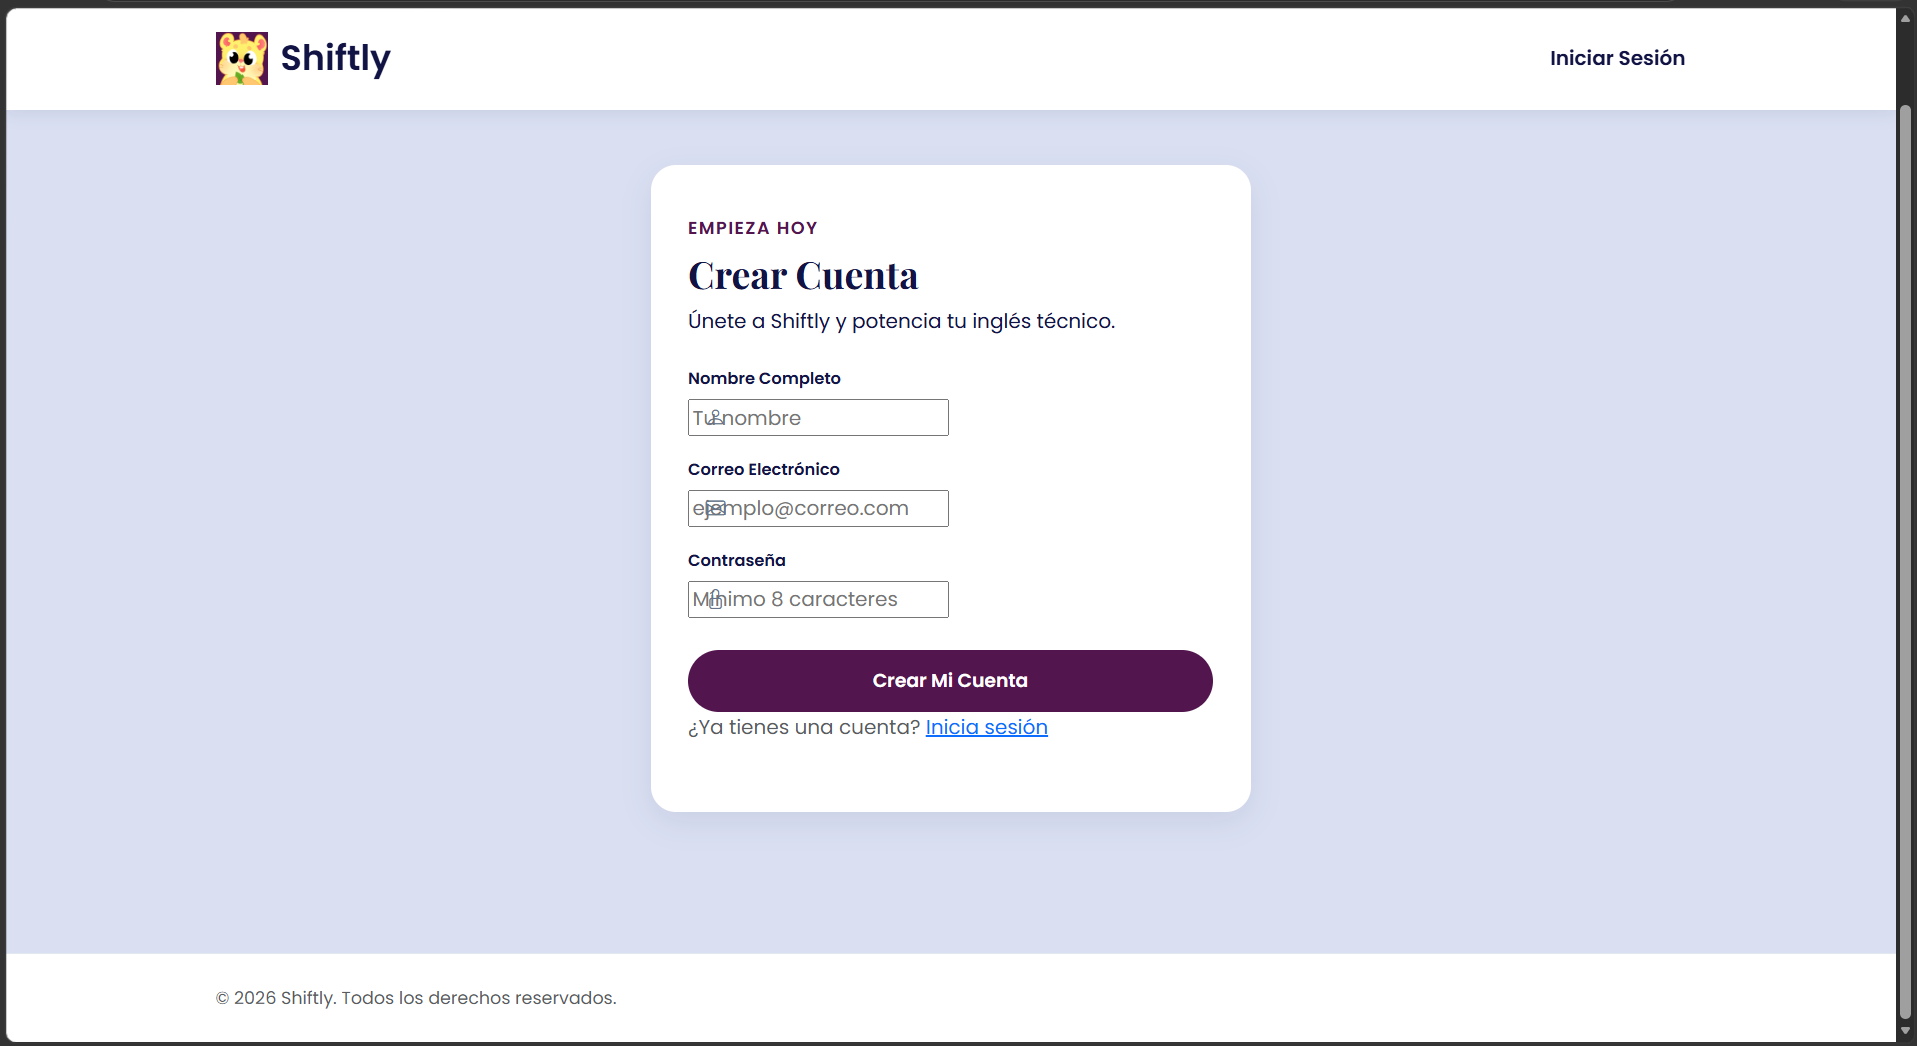
\includegraphics[width=\textwidth]{registro.png}
\caption{Interfaz de registro de usuario de SHIFTLY.}
\label{fig:registro}
\end{figure}
\subsubsection{Selección de áreas de aprendizaje}
La interfaz de selección de áreas de aprendizaje permite al usuario elegir
el área de inglés que desea aprender de acuerdo con sus intereses. Esta
sección presenta diferentes opciones mediante tarjetas interactivas y
proporciona un mecanismo para seleccionar una de ellas antes de continuar
con el proceso de aprendizaje\\
\textbf{Barra de navegación}\\
La parte superior de la interfaz contiene una barra de navegación que
incluye el nombre de SHIFTLY, el logotipo de la aplicación y las opciones
de navegación Inicio, Aprender, Mi perfil y Ayuda. Estos elementos forman
parte de la estructura general de navegación de la aplicación web\\
\textbf{Encabezado de la sección}\\
La sección presenta el título ``¿Qué inglés quieres aprender?'' junto con
un texto introductorio que explica al usuario que puede elegir un área de
aprendizaje para adaptar el contenido de acuerdo con sus intereses\\
\textbf{Áreas de aprendizaje}\\
La interfaz presenta cinco áreas de aprendizaje mediante tarjetas
individuales:
\begin{itemize}
\item \textbf{Programación:} presenta contenido de inglés enfocado en tecnología, desarrollo y mundo digital.
\item \textbf{Gastronomía:} presenta vocabulario, expresiones y situaciones relacionadas con el mundo culinario.
\item \textbf{Turismo:} presenta contenido relacionado con viajes, hoteles, atención al cliente y experiencias turísticas.
\item \textbf{Negocios:} presenta contenido orientado a ambientes profesionales, empresariales y comunicación laboral.
\item \textbf{Inglés cotidiano:} presenta expresiones y vocabulario relacionados con situaciones diarias de la vida real.
\end{itemize}
\textbf{Botones de selección}\\
Cada tarjeta contiene un botón denominado ``Seleccionar'' al presionar
este botón, el área correspondiente se identifica visualmente como la
opción seleccionada, cuando existe un área seleccionada, se permite continuar con el proceso de aprendizaje la integración con la siguiente interfaz se realizará posteriormente como parte del desarrollo colaborativo del proyecto.\\
\textbf{Botón Continuar}\\
La interfaz cuenta con un botón ``Continuar'' que permite avanzar al
siguiente paso del proceso, antes de continuar se verifica que el usuario
haya seleccionado un área de aprendizaje si el usuario intenta continuar sin seleccionar
un área, la aplicación muestra un mensaje solicitando realizar una selección, cuando existe un
área seleccionada, se permite continuar con el proceso de aprendizaje, la siguiente etapa del flujo corresponde al diagnóstico inicial, cuya integración con esta interfaz se realizará posteriormente como parte del desarrollo colaborativo del proyecto.
\begin{figure}[H]
\centering
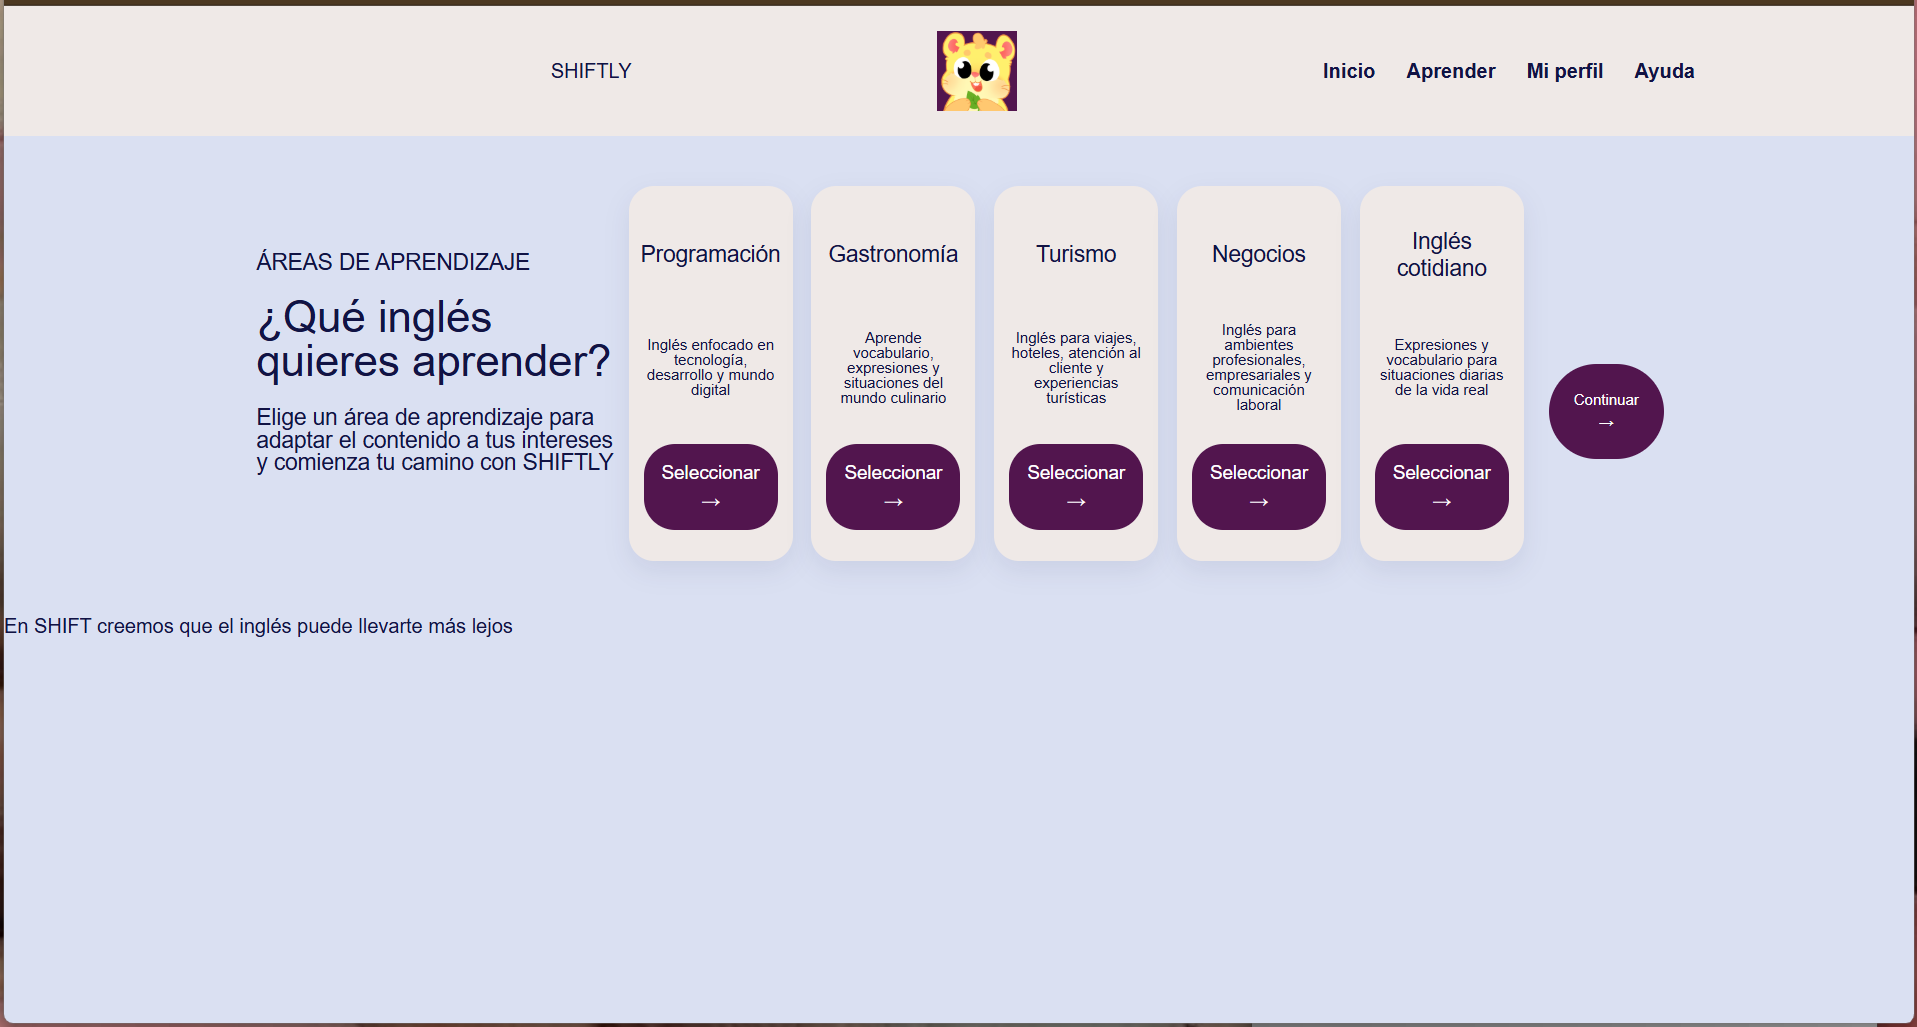
\includegraphics[width=\textwidth]{seleccion areas.png}
\caption{Interfaz de selección de áreas de aprendizaje en SHIFTLY}
\label{fig:seleccion areas}
\end{figure}
\subsubsection{Diagnóstico inicial}
\textbf{Descripción}
La interfaz de diagnóstico inicial permite al usuario realizar una
evaluación para conocer su nivel actual de inglés. La pantalla presenta
una serie de preguntas con diferentes opciones de respuesta y muestra el
avance del usuario durante el diagnóstico.
\textbf{Barra de navegación}
La parte superior de la interfaz contiene la barra de navegación de
SHIFTLY. En ella se muestra el logotipo y nombre de la aplicación, así
como las opciones ``Inicio'', ``Aprender'', ``Mi perfil'' y ``Ayuda''.
\textbf{Encabezado del diagnóstico}
La sección principal presenta la etiqueta ``TEST DE DIAGNÓSTICO'' y el
título ``Descubre tu nivel de inglés''. También incluye un texto
introductorio que explica al usuario que debe responder las preguntas
para conocer su nivel actual y recibir recomendaciones de aprendizaje.
\textbf{Indicador de progreso}
La interfaz incorpora una sección denominada ``Progreso'' que permite
visualizar el avance del usuario dentro del diagnóstico. En la captura se
muestra el indicador ``1 de 5'', acompañado de una barra de progreso que
representa el avance de la evaluación.
\textbf{Pregunta de diagnóstico}
La pantalla presenta la ``Pregunta 1'' dentro de una tarjeta de
contenido. La pregunta mostrada es ``Choose the correct option:'' y se
presentan diferentes alternativas para responderla.
\begin{itemize}
\item \textbf{She are a student.}
\item \textbf{She is a student.}
\item \textbf{She am a student.}
\item \textbf{She be a student.}
\end{itemize}
Las opciones permiten al usuario identificar la respuesta que considera
correcta para continuar con el diagnóstico.
\textbf{Pie de página}
En la parte inferior de la interfaz se presenta el mensaje ``En Shiftly
creemos que el inglés puede llevarte más lejos'', utilizado como elemento
informativo de la aplicación.
\textbf{Evidencia}
La siguiente captura muestra la interfaz del diagnóstico inicial de
SHIFTLY
\begin{figure}[H]
\centering
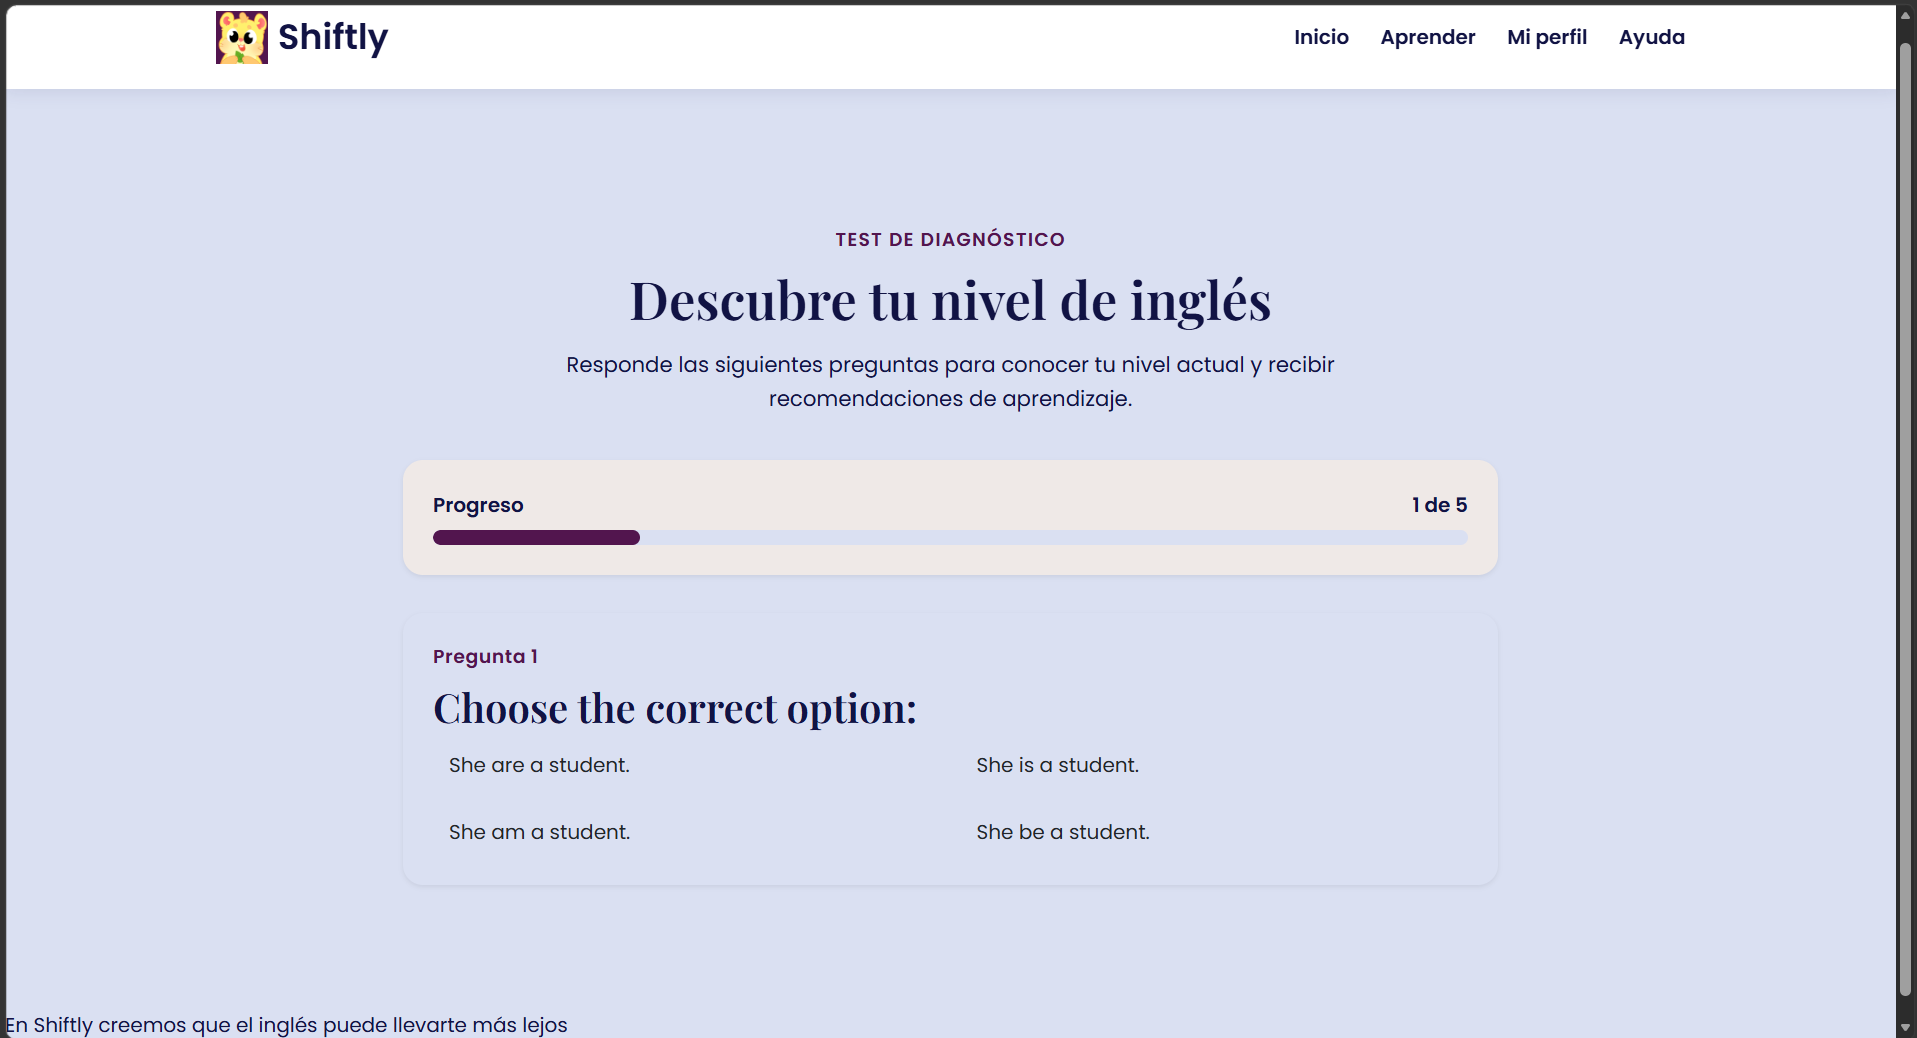
\includegraphics[width=\textwidth]{diagnostico.png}
\caption{Interfaz de diagnóstico inicial de SHIFTLY.}
\label{fig:diagnostico}
\end{figure}
\subsubsection{Vaneza Lugo Ramírez}
\textbf{Tarjetas de vocabulario}
Esta interfaz corresponde a las tarjetas de aprendizaje utilizadas para
presentar vocabulario en inglés, incluyendo información relacionada con
las palabras y su aprendizaje.
\textbf{Evidencia:}
\textit{En este apartado se colocará la captura de las tarjetas de
vocabulario.}
\vspace{0.5cm}
\textbf{Biblioteca y repaso}
Esta interfaz corresponde a la sección destinada al repaso de contenidos
y vocabulario previamente estudiado por el usuario.
\textbf{Evidencia:}
\textit{En este apartado se colocará la captura de la biblioteca y sección
de repaso.}
\subsubsection{Brian Jael Juárez Rodríguez}
\textbf{Ejercicios interactivos}
Esta interfaz corresponde a las actividades interactivas utilizadas para
que el usuario practique los contenidos de aprendizaje mediante diferentes
ejercicios.
\textbf{Evidencia:}
\textit{En este apartado se colocará la captura de los ejercicios
interactivos.}
\subsubsection{Julio}
\textbf{Mapa de lecciones}
Esta interfaz representa la ruta de aprendizaje del usuario mediante un
mapa o estructura de lecciones.
\textbf{Evidencia:}
\textit{En este apartado se colocará la captura del mapa de lecciones.}
\vspace{0.5cm}
\textbf{Siguiente lección recomendada}
Esta interfaz corresponde a la sección encargada de mostrar al usuario una
recomendación de la siguiente lección dentro de su proceso de aprendizaje.
\textbf{Evidencia:}
\textit{En este apartado se colocará la captura de la siguiente lección
recomendada.}
\subsection{Control de versiones}
El proyecto utiliza Git y GitHub para administrar el código fuente y
mantener un registro de los cambios realizados durante el desarrollo.
El trabajo se organizó mediante ramas para desarrollar las diferentes
funcionalidades de manera independiente antes de integrarlas al proyecto
principal.
\textbf{Evidencia:}
\textit{En este apartado se colocará la captura del repositorio y las ramas
utilizadas.}
\subsection{Commits}
Durante el desarrollo se realizaron commits descriptivos para registrar
los avances realizados en la aplicación web.
En el caso de la interfaz de selección de áreas de aprendizaje se
realizaron diferentes commits relacionados con la estructura de la
pantalla, las áreas de aprendizaje, la selección de áreas y la validación
del botón de continuar.
\textbf{Evidencia:}
\textit{En este apartado se colocará la captura del historial de commits.}
\subsection{Pull Request}
Después de completar el desarrollo de la funcionalidad correspondiente, se
creó un Pull Request para solicitar la integración de los cambios a la
rama principal del proyecto.
\textbf{Evidencia:}
\textit{En este apartado se colocará la captura del Pull Request.}
\subsection{Tablero Kanban}
El desarrollo del proyecto se organizó mediante un tablero Kanban para
dar seguimiento al avance de las actividades asignadas a los integrantes
del equipo.
\textbf{Evidencia:}
\textit{En este apartado se colocará la captura del tablero Kanban.}
\subsection{Pruebas responsive}
La aplicación web SHIFTLY se diseñó considerando diferentes tamaños de
pantalla. Para comprobar su adaptación se realizarán capturas de la
aplicación en computadora y en dispositivos móviles.
\textbf{Evidencia:}
\textit{En este apartado se colocarán las capturas de la aplicación en
computadora y teléfono móvil.}